\subsection{UML-Diagramm}

\begin{figure}[hbtp]
\centering
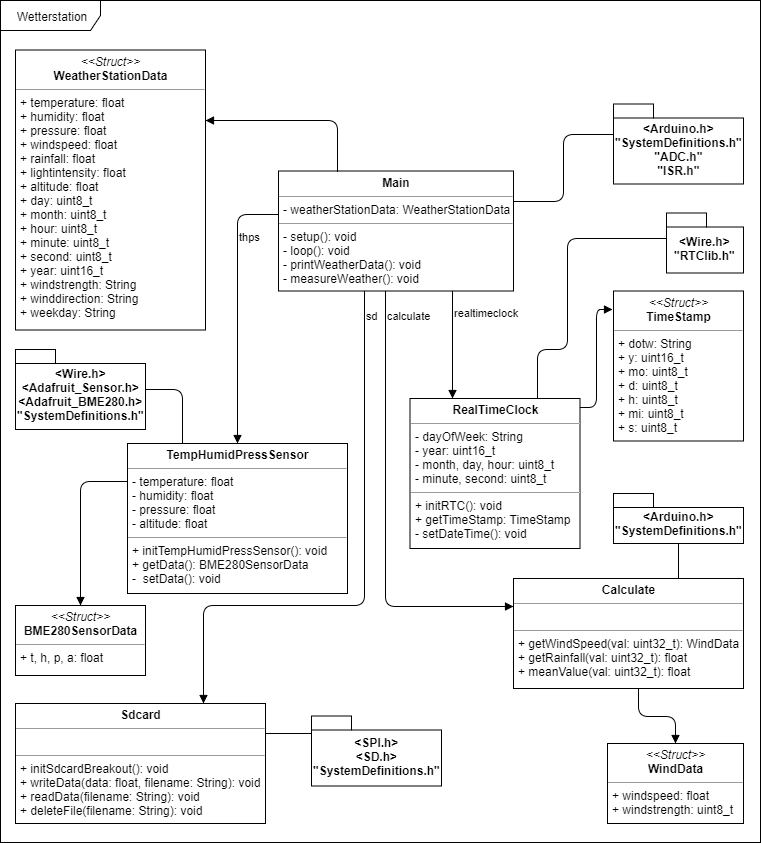
\includegraphics[width=\textwidth]{graphics/UML/UML_Diagramm_picture.PNG}
\caption{UML-Diagramm der Wetterstation}
\label{fig:uml_diagramm}
\end{figure}

Das in der Abbildung \ref{fig:uml_diagramm} dargestellte UML-Diagramm soll den Aufbau und die logischen Zusammenhänge der Firmware visualisieren. Darin wird gezeigt, welche Headerfiles bei den Klassen benötigt werden. Zudem sind die Attribute, wie auch die Funktionen mit ihren Access Specifier, Argumenten und Rückgabewerten aufgelistet. \\

Durch diese Struktur ist es möglich, adaptiv mehrere Komponenten hinzuzufügen und anzupassen. Zudem könnten somit auch mehrere Sensoren vom gleichen Typ ohne grossen weiteren Aufwand implementiert werden.\\

In der Klasse \textbf{TempHumidPressSensor} werden die Temperatur, Lufdruck und relative Luftfeuchtigkeit vom BME280 gelesen und in das Struct BME280SensorData geschrieben. Diese können dann vom \textbf{Main} über die Funktion \textit{getData()} aufgerufen werden. Über die Klasse \textbf{RealTimeClock} können die Zeitdaten vom DS3231 und zu den Messwerten zugerordnet werden. Mittels einer Klasse \textbf{Calculate} sollen notwendige Berechnungen vom restlichen Programm getrennt werden. Wenn das Programm startet, wird zuerst das \textit{setup()} aufgerufen und danach befindet sich das Programm in der Endlosschlaufe \textit{loop()}. Dieser Stil ist typisch für die Arduino IDE, wie im Kapitel \ref{subsec:dev_envir} bereits erwähnt worden ist, wird in diesem Projekt in zwei Development Environments gearbeitet.